\documentclass[a4paper,12pt]{article} 
\usepackage[T2A]{fontenc}			
\usepackage[utf8]{inputenc}			
\usepackage[english,russian]{babel}	
\usepackage{amsmath,amsfonts,amssymb,amsthm,mathtools} 
\usepackage[colorlinks, linkcolor = blue]{hyperref}
\usepackage{upgreek}
\usepackage[left=2cm,right=2cm,top=2cm,bottom=3cm,bindingoffset=0cm]{geometry}
\usepackage{multirow}
\usepackage{graphicx}
\usepackage{xcolor}
\usepackage{multirow}
\usepackage{pgfplots}
\usepackage{pgfplotstable}
\pgfplotsset{compat=1.9}

\pgfplotstableset{ %
        create on use/SquareLight/.style={
                create col/expr={\thisrow{Dark}}}
}

\author{Шелихов Дмитрий\\Группа Б01-305}

\title{\textbf{Работа 3.5.1\\Изучение плазмы газового разряда в неоне}} 
\date{\today}

\begin{document} 

\maketitle

\par\textbf{Цель работы: }Снять вольт-амперную характеристику тлеющего разряда и зондовые характеристики при разных токах разряда и по результатам измерений рассчитать концентрацию и температуру электронов в плазме, плазменную частоту, поляризационную длину, дебаевский радиус экранирования и степень ионизации.

\par\textbf{В работе используются: } стеклянная газоразрядная трубка, наполненная неоном, высоковольтный источник питания, источник питания постоянного тока, делитель напряжения, резистор, потенциометр, амперметры, вольтметры, переключатели. 

\par\textbf{Экспериментальная установка}

\begin{figure}[htp]
\center{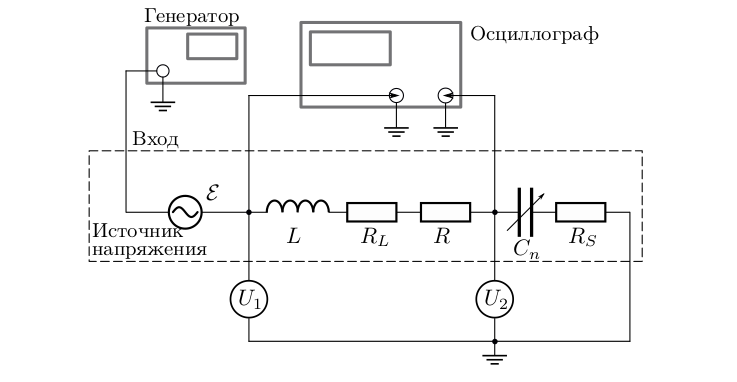
\includegraphics[width=.8\textwidth]{1.png}}
\caption{Схема установки для исследования газового разряда}
\end{figure}

Стекланная газоразрядная трубка имеет холодный (ненагреваемый) полый катод, три анода и геттерный узел - стеклянный баллон, на внутреннюю поверхность которого напылена газопоглощающая плёнка (геттер). Трубка наполнена изотопом неона $^{22}{Ne}$ при давлении 2 мм рт. ст.
При подключении к ВИП анода 1 между ним и катодом возникает газовый разряд. Ток разряда и падение напряжения измеряются с помощью мультиметров (A1 и U1 соотв.).
При подключении к ВИП анода 2 рязряд возникает в пространстве между катодом и анодом 2, где находится двойной зонд, используемый для диагностики плазмы положительного столба. \\

Переключатель П2 позволяет менять полярность напряжения на зондах. \\

Зонд изготовлен из молибденовой проволоки диаметром d и имеют длину l. 

\par\textbf{Ход работы:}
\par\textbf{I. Вольт-амперная характеристика разряда:}
\par1) Подготовим приборы к работе:
\begin{itemize}
\item Установим переключатель П1 в положение "Анод 1".
\item Поставим ручку регулировки выходного напряжения ВИП в крайнее левое положение и включим прибор в сеть 
\item Подготовим к работе мультиметр V1 
\end{itemize}

\parПлавно увеличивая выходное напряжение ВИП, определим напряжение зажигания разряда $U_{\text{заж}}$ (показания вольтметра V1 перед зажиганием) \\

\begin{tabular}{|c|}
	\hline
	$U_{\text{заж}} \approx$ 220 В \\
	\hline
\end{tabular}

\par 2) С помощью вольтметра $V_1$ и амперметра $A_1$ снимем вольт-амперную характеристику разряда $I_p(U_p)$. Ток разряда $I_p$ будем изменять в диапазоне от 0,5 мА до $\approx$ 5мА. 

\begin{tabular}{|c|c|}
	\hline
	\multicolumn{2}{|c|}{\text{При нарастании тока}}\\
	\hline
	$U_p$, В & $I_p$, мА \\
	\hline
	34.93 $\pm$ 0.05 & 0.53 $\pm$ 0.01 \\
	\hline 
	33.02 $\pm$ 0.05 & 1.19 $\pm$ 0.01 \\
	\hline
	28.44 $\pm$ 0.05 & 1.51 $\pm$ 0.01 \\
	\hline
	21.88 $\pm$ 0.05 & 2.03 $\pm$ 0.01 \\
	\hline
	17.95 $\pm$ 0.05 & 2.54 $\pm$ 0.01 \\
	\hline
	15.62 $\pm$ 0.05 & 3.02 $\pm$ 0.01 \\
	\hline
	14.00 $\pm$ 0.05 & 3.51 $\pm$ 0.01 \\
	\hline
	11.16 $\pm$ 0.05 & 4.08 $\pm$ 0.01 \\
	\hline
	8.73 $\pm$ 0.05 & 4.50 $\pm$ 0.01 \\
	\hline
\end{tabular}
\qquad
\begin{tabular}{|c|c|}
	\hline
	\multicolumn{2}{|c|}{\text{При убывании тока}}\\
	\hline
	$U_p$, В & $I_p$, мА \\
	\hline
	7.87 $\pm$ 0.05 & 4.63 $\pm$ 0.01 \\
	\hline
	11.35 $\pm$ 0.05 & 4.01 $\pm$ 0.01 \\
	\hline
	13.93 $\pm$ 0.05 & 3.48 $\pm$ 0.01 \\
	\hline
	15.18 $\pm$ 0.05 & 3.07 $\pm$ 0.01 \\
	\hline
	18.00 $\pm$ 0.05 & 2.51 $\pm$ 0.01 \\
	\hline
	21.58 $\pm$ 0.05 & 2.04 $\pm$ 0.01 \\
	\hline
	27.39 $\pm$ 0.05 & 1.55 $\pm$ 0.01 \\
	\hline
	33.84 $\pm$ 0.05 & 1.02 $\pm$ 0.01 \\
	\hline
	34.98 $\pm$ 0.05 & 0.52 $\pm$ 0.01 \\
	\hline
\end{tabular}

\par 3) Построим вольт-амперную характеристику разряда в координатах $I_p$($U_p$). Данные возьмем при убывании тока. \\

\pgfplotstableread{
x			y			y-min		y-max		x-min		x-max
7.87		4.63		0.01		0.01		0.05		0.05
11.35		4.01		0.01		0.01		0.05		0.05
13.93		3.48		0.01		0.01		0.05		0.05
15.18		3.07		0.01		0.01		0.05		0.05
18.00		2.51		0.01		0.01		0.05		0.05
21.58		2.04		0.01		0.01		0.05		0.05
27.39		1.55		0.01		0.01		0.05		0.05
33.84		1.02		0.01		0.01		0.05		0.05
34.98		0.52		0.01		0.01		0.05		0.05
}{\mytable}

\resizebox{\columnwidth}{!}{
\begin{tikzpicture}
\begin{axis} [
	title = $I_p(U_p)$,
	xlabel = {$U_p$, В},
	ylabel = {$I_p$, мА},
	minor tick num = 2,
	grid = major
]

\addplot +[mark options = {scale = 0.1,}]
	plot [error bars/.cd, y dir=both, x dir=both, y explicit, x explicit]
	table [y error plus=y-max, y error minus=y-min, x error plus=x-max, x error minus=x-min] {\mytable};

\addplot +[mark options = {scale = 0,}]
	table[row sep=\\,				%аппроксимация
   y={create col/linear regression={y=Y}}]
    {
   		X Y\\
   		21.58		2.04 \\
		27.39       1.55 \\
    };
	\addlegendentry{
        dU/dI$\approx \pgfmathprintnumber{\pgfplotstableregressiona}$, кОм}
\end{axis}
\end{tikzpicture}
}

\par По наклону кривой определим максимальное дифференциальное сопротивление разряда $R_{\text{диф}}$ = dU/dI. Для этого возьмём участок графика, с наименьшим наклоном.

\begin{tabular}{|c|c|}
	\hline
	$R_{\text{диф}}$ = (11.9 $\pm$ 0.7) кОм\\
	\hline	
\end{tabular}

\par Проделаем то же самое для данных при возрастании тока: 

\pgfplotstableread{
x			y			y-min		y-max		x-min		x-max
8.73		4.50		0.01		0.01		0.05		0.05
11.16		4.08		0.01		0.01		0.05		0.05
14.00		3.51		0.01		0.01		0.05		0.05
15.62		3.02		0.01		0.01		0.05		0.05
17.95		2.54		0.01		0.01		0.05		0.05
21.88		2.03		0.01		0.01		0.05		0.05
28.44		1.51		0.01		0.01		0.05		0.05
33.02		1.19		0.01		0.01		0.05		0.05
34.93		0.53		0.01		0.01		0.05		0.05
}{\mytable}

\resizebox{\columnwidth}{!}{
\begin{tikzpicture}
\begin{axis} [
	title = $I_p(U_p)$,
	xlabel = {$U_p$, В},
	ylabel = {$I_p$, мА},
	minor tick num = 2,
	grid = major
]

\addplot +[mark options = {scale = 0.1,}]
	plot [error bars/.cd, y dir=both, x dir=both, y explicit, x explicit]
	table [y error plus=y-max, y error minus=y-min, x error plus=x-max, x error minus=x-min] {\mytable};

\addplot +[mark options = {scale = 0,}]
	table[row sep=\\,				%аппроксимация
   y={create col/linear regression={y=Y}}]
    {
   		X Y\\
		28.44		1.51 \\
		21.88       2.03 \\
    };
	\addlegendentry{
        dI/dU$\approx \pgfmathprintnumber{\pgfplotstableregressiona}$, $10^{-3}{\text{Ом}}^{-1}$}
\end{axis}
\end{tikzpicture}
}

\par Аналогично выбираем часть графика с наименьшим наклоном и находим $R_{\text{диф}}$:

\begin{tabular}{|c|c|}
	\hline
	$R_{\text{диф}}$ = (12.6 $\pm$ 0.7) кОм\\
	\hline
\end{tabular}

\par Таким образом получаем 2 значения для $R_{\text{диф}}$, которые совпадают в пределах абсолютной погрешности. Усредним значение и далее будем использовать именно его: 

\begin{tabular}{|c|c|c|}
	\hline
	$R_{\text{диф}^{\text{нараст}}}$, кОм & $R_{\text{диф}^{\text{убыв}}}$, кОм & $R_{\text{диф}}^{\text{сред}}$, кОм \\
	\hline
	12.6 $\pm$ 0.7 & 11.9 $\pm$ 0.7 & 12.3 $\pm$ 0.7 \\
	\hline
\end{tabular}

\par Полученный график соответствует поднормальному участку ВАХ (см. приложение в учебнике). При токе $I_p \approx$ 4.5 мА кривая переходит в вертикальный участок ГВ графика из приложения (темный таунсендовский разряд. Токи и степень ионизации еще малы, чтобы вызвать свечение, но критерий Таунсенда выполнен). 

\par \textbf{Зондовые характеристики}

\par 4) Уменьшим напряжение ВИП до нуля и переведем П1 в положение "Анод 2", П2 в положение "+". Подготовим мультиметры А2 и U2, включим приборы в сеть. 

\par 5) Плавно увеличивая напряжение на ВИП дойдем до возникновения разряда и установим разрядный ток $I_p = $ (4.73 $\pm$ 0.01)мА. Включим в сеть источник питания GPS и установим на нем напряжение $U_2\approx$25В. При помощи потенциометра установим на зонде максимальное напряжение $U_2\approx$25В. 

\par 6) С помощью мультиметров $A_2$ и $U_2$ снимем ВАХ двойного зонда $I_{\text{з}}$($U_{\text{з}}$) (в диапазоне +25В до -25В) при фиксированном тока разряда $I_p$.

\begin{tabular}{|c|c|c|}
	\hline
	$U_{\text{з}}$, В & $I_{\text{з}}$, мкА &  $I_p$, мА \\
	\hline
	-25.01 $\pm$ 0.05 & -115.9 $\pm$ 0.1 & \multirow{21}{*}{4.73 $\pm$ 0.01}\\
	\cline{1-2} 
	-22.25 $\pm$ 0.05 & -113.4 $\pm$ 0.1 & \\
	\cline{1-2}
	-18.95 $\pm$ 0.05 & -108.5 $\pm$ 0.1 & \\
	\cline{1-2}
	-16.02 $\pm$ 0.05 & -101.1 $\pm$ 0.1 & \\
	\cline{1-2}
	-13.15 $\pm$ 0.05 & -91.2 $\pm$ 0.1 & \\
	\cline{1-2}
	-10.58 $\pm$ 0.05 & -79.8 $\pm$ 0.1 & \\
	\cline{1-2}
	-7.99 $\pm$ 0.05 & -66.6 $\pm$ 0.1 & \\
	\cline{1-2}
	-6.00 $\pm$ 0.05 & -54.5 $\pm$ 0.1 & \\
	\cline{1-2}
	-4.03 $\pm$ 0.05 & -41.8 $\pm$ 0.1 & \\
	\cline{1-2}
	-2.11 $\pm$ 0.05 & -27.2 $\pm$ 0.1 & \\
	\cline{1-2}
	-0.55 $\pm$ 0.05 & -15.0 $\pm$ 0.1 & \\
	\cline{1-2}
	0.51 $\pm$ 0.05 & 17.6 $\pm$ 0.1 & \\
	\cline{1-2}
	2.11 $\pm$ 0.05 & 27.8 $\pm$ 0.1 & \\
	\cline{1-2}
	4.17 $\pm$ 0.05 & 40.9 $\pm$ 0.1 & \\
	\cline{1-2}
	5.92 $\pm$ 0.05 & 50.6 $\pm$ 0.1 & \\
	\cline{1-2}
	7.93 $\pm$ 0.05 & 60.7 $\pm$ 0.1 & \\
	\cline{1-2}
	10.05 $\pm$ 0.05 & 70.7 $\pm$ 0.1 & \\
	\cline{1-2}
	12.05 $\pm$ 0.05 & 77.5 $\pm$ 0.1 & \\
	\cline{1-2}
	15.07 $\pm$ 0.05 & 86.4 $\pm$ 0.1 & \\
	\cline{1-2}
	18.31 $\pm$ 0.05 & 92.7 $\pm$ 0.1 & \\
	\cline{1-2}
	21.00 $\pm$ 0.05 & 96.0 $\pm$ 0.1 & \\
	\hline
\end{tabular}

\par 7) Построим зондовую характеристику, предварительно отцентрировав кривую    ($I_0$ = $\Sigma I/2$). Найдем ток насыщения $I_{i\text{н}}$ из пересечения асимптоты к верхней и нижней части графика с осью U = 0, а также величину $\frac{dI}{dU}$ при U = 0.

\pgfplotstableread{
x			y			y-min		y-max		x-min		x-max
-22.25		-113.4		0.1		0.1		0.05		0.05
-18.95		-108.5		0.1		0.1		0.05		0.05
-16.02		-101.1		0.1		0.1		0.05		0.05
-13.15		-91.2		0.1		0.1		0.05		0.05
-10.58		-79.8		0.1		0.1		0.05		0.05
-7.99		-66.6		0.1		0.1		0.05		0.05
-6			-54.5 		0.1		0.1		0.05		0.05
-4.03		-41.8		0.1		0.1		0.05		0.05
-2.11		-27.2		0.1		0.1		0.05		0.05
-0.55		-15			0.1		0.1		0.05		0.05
0.51		17.6		0.1		0.1		0.05		0.05
2.11		27.8		0.1		0.1		0.05		0.05
4.17		40.9		0.1		0.1		0.05		0.05
5.92		50.6		0.1		0.1		0.05		0.05
7.93		60.7		0.1		0.1		0.05		0.05
10.05		70.7		0.1		0.1		0.05		0.05
12.05		77.5		0.1		0.1		0.05		0.05	
15.07		86.4		0.1		0.1		0.05		0.05
18.31		92.7		0.1		0.1		0.05		0.05
21			96			0.1		0.1		0.05		0.05
}{\mytable}

\resizebox{\columnwidth}{!}{
\begin{tikzpicture}
\begin{axis} [
	title = $I_{\text{з}}(U_{\text{з}})$,
	xlabel = {$U_{\text{з}}$, В},
	ylabel = {$I_{\text{з}}$, мкА},
	minor tick num = 2,
	grid = major
]

\addplot +[mark options = {scale = 0.1,}]
	plot [error bars/.cd, y dir=both, x dir=both, y explicit, x explicit]
	table [y error plus=y-max, y error minus=y-min, x error plus=x-max, x error minus=x-min] {\mytable};

\addplot +[mark options = {scale = 0,}]
	table[row sep=\\,				%аппроксимация
   y={create col/linear regression={y=Y}}]
    {
   		X Y\\
		-2.11       -27.2\\
		-0.55       -15\\
		0.51        17.6\\
		2.11        27.8\\
    };
\addplot +[mark options = {scale = 0,}]
    table[row sep=\\,               %аппроксимация
   y={create col/linear regression={y=Y}}]
    {
        X Y\\
       	-22.25	-113.4\\
        -18.95	-108.5\\
        -16.02	-101.1\\
    };
\addplot +[mark options = {scale = 0,}]
    table[row sep=\\,               %аппроксимация
    y={create col/linear regression={y=Y}}]
     {
         X Y\\
         15.07       86.4\\
		 18.31       92.7\\
		 21          96\\  
     };
\end{axis}
\end{tikzpicture}
}
\par Откуда:\\
\begin{center}
\begin{tabular}{|c|c|c|c|}
	\hline
	$\frac{dI}{dU}$, мкА/В & $I_{i\text{н}}^{\text{асимптота снизу}}$, мкА & $I_{i\text{н}}^{\text{асимптота сверху}}$, мкА & $I_p$, мА \\
	\hline
	14.08 $\pm$ 0.61 & -70.2 $\pm$ 2.8  & 62.2 $\pm$ 2.6 & 4.73 $\pm$ 0.01 \\
	\hline
\end{tabular}
\end{center}

Усредним полученное значение для $I_{i\text{н}}$: (66.2 $\pm$ 2.7) мкА. \\

Определим $\Delta U$ между точками 1 и 2: \begin{tabular}{|c|} \hline $\Delta U = 4.42 \pm 0.38$ В.\\ \hline \end{tabular}

\par8) Аналогичные измерения проделаем для токов разряда $I_p$ = (2.99 $\pm$ 0.01) мА и $I_p$ = (1.49 $\pm$ 0.01) мА.\\

\begin{tabular}{|c|c|c|}
	\hline
	$U_{\text{з}}$, В & $I_{\text{з}}$, мкА &  $I_p$, мА \\
	\hline
	-24.99 $\pm$ 0.05 & -59.1 $\pm$ 0.1 & \multirow{22}{*}{2.99 $\pm$ 0.01}\\
	\cline{1-2}
	-22.31 $\pm$ 0.05 & -57.7 $\pm$ 0.1 & \\
	\cline{1-2}
	-19.16 $\pm$ 0.05 & -55.8 $\pm$ 0.1 & \\
	\cline{1-2}
	-15.75 $\pm$ 0.05 & -52.9 $\pm$ 0.1 & \\
	\cline{1-2}
	-12.16 $\pm$ 0.05 & -47.4 $\pm$ 0.1 & \\
	\cline{1-2}
	-10.09 $\pm$ 0.05 & -43.1 $\pm$ 0.1 & \\
	\cline{1-2}
	-8.19 $\pm$ 0.05 & -37.8 $\pm$ 0.1 & \\
	\cline{1-2}
	-6.09 $\pm$ 0.05 & -30.5 $\pm$ 0.1 & \\
	\cline{1-2}
	-4.06 $\pm$ 0.05 & -22.1 $\pm$ 0.1 & \\
	\cline{1-2}
	-2.08 $\pm$ 0.05 & -13.3 $\pm$ 0.1 & \\
	\cline{1-2}
	-0.53 $\pm$ 0.05 & -4.7 $\pm$ 0.1 & \\
	\cline{1-2}
	0.66 $\pm$ 0.05 & 7.3 $\pm$ 0.1 & \\
	\cline{1-2}
	2.11 $\pm$ 0.05 & 14.7 $\pm$ 0.1 & \\
	\cline{1-2}
	4.30 $\pm$ 0.05 & 24.6 $\pm$ 0.1 & \\
	\cline{1-2}
	6.01 $\pm$ 0.05 & 31.1 $\pm$ 0.1 & \\
	\cline{1-2}
	8.11 $\pm$ 0.05 & 37.8 $\pm$ 0.1 & \\
	\cline{1-2}
	10.32 $\pm$ 0.05 & 43.0 $\pm$ 0.1 & \\
	\cline{1-2}
	13.25 $\pm$ 0.05 & 48.1 $\pm$ 0.1 & \\
	\cline{1-2}
	16.67 $\pm$ 0.05 & 51.7 $\pm$ 0.1 & \\
	\cline{1-2}
	19.34 $\pm$ 0.05 & 53.5 $\pm$ 0.1 & \\
	\cline{1-2}
	22.58 $\pm$ 0.05 & 55.3 $\pm$ 0.1 & \\
	\cline{1-2}
	24.98 $\pm$ 0.05 & 56.5 $\pm$ 0.1 & \\
	\hline
\end{tabular}

\pgfplotstableread{
x			y			y-min		y-max		x-min		x-max
-24.99		-59.1		0.1		0.1		0.05		0.05
-22.31		-57.7		0.1		0.1		0.05		0.05
-19.16		-55.8		0.1		0.1		0.05		0.05
-15.75		-52.9		0.1		0.1		0.05		0.05
-12.16		-47.4		0.1		0.1		0.05		0.05
-10.09		-43.1		0.1		0.1		0.05		0.05
-8.19		-37.8 		0.1		0.1		0.05		0.05
-6.09		-30.5		0.1		0.1		0.05		0.05
-4.06		-22.1		0.1		0.1		0.05		0.05
-2.08		-13.3		0.1		0.1		0.05		0.05
-0.53		-4.7		0.1		0.1		0.05		0.05
0.66		7.3			0.1		0.1		0.05		0.05
2.11		14.7		0.1		0.1		0.05		0.05
4.30		24.6		0.1		0.1		0.05		0.05
6.01		31.1		0.1		0.1		0.05		0.05
8.11		37.8		0.1		0.1		0.05		0.05
10.32		43.0		0.1		0.1		0.05		0.05
13.25		48.1		0.1		0.1		0.05		0.05
16.67		51.7		0.1		0.1		0.05		0.05
19.34		53.5		0.1		0.1		0.05		0.05
22.58		55.3		0.1		0.1		0.05		0.05
24.98		56.5		0.1		0.1		0.05		0.05
}{\mytable}

\resizebox{\columnwidth}{!}{
\begin{tikzpicture}
\begin{axis} [
	title = $I_{\text{з}}(U_{\text{з}})$,
	xlabel = {$U_{\text{з}}$, В},
	ylabel = {$I_{\text{з}}$, мкА},
	minor tick num = 2,
	grid = major
]

\addplot +[mark options = {scale = 0.1,}]
	plot [error bars/.cd, y dir=both, x dir=both, y explicit, x explicit]
	table [y error plus=y-max, y error minus=y-min, x error plus=x-max, x error minus=x-min] {\mytable};

\addplot +[mark options = {scale = 0,}]
	table[row sep=\\,				%аппроксимация
   y={create col/linear regression={y=Y}}]
    {
   		X Y\\
    	-2.08       -13.3\\
		-0.53       -4.7\\
		0.66        7.3\\
		2.11        14.7\\
    };
\addplot +[mark options = {scale = 0,}]
    table[row sep=\\,               %аппроксимация
   y={create col/linear regression={y=Y}}]
    {
        X Y\\
      	-24.99      -59.1\\
      	-22.31      -57.7\\
		-19.16      -55.8\\
    };
\addplot +[mark options = {scale = 0,}]
    table[row sep=\\,               %аппроксимация
    y={create col/linear regression={y=Y}}]
     {
         X Y\\
         19.34       53.5\\
		 22.58       55.3\\
		 24.98       56.5\\
     };
\end{axis}
\end{tikzpicture}
}
\par Откуда:\\
\begin{center}
\begin{tabular}{|c|c|c|c|}
	\hline
	$\frac{dI}{dU}$, мкА/В & $I_{i\text{н}}^{\text{асимптота снизу}}$, мкА & $I_{i\text{н}}^{\text{асимптота сверху}}$, мкА & $I_p$, мА \\
	\hline
	6.94 $\pm$ 0.30 & -45.0 $\pm$ 1.8  & 43.2 $\pm$ 1.8 & 2.99 $\pm$ 0.01 \\
	\hline
\end{tabular}
\end{center}

Усредним полученное значение для $I_{i\text{н}}$: (44.1 $\pm$ 1.8) мкА. \\

Определим $\Delta U$ между точками 1 и 2: \begin{tabular}{|c|} \hline $\Delta U = 6.90 \pm 0.59 $ В.\\ \hline \end{tabular}

\begin{tabular}{|c|c|c|}
	\hline
	$U_{\text{з}}$, В & $I_{\text{з}}$, мкА &  $I_p$, мА \\
	\hline
	-25.00 $\pm$ 0.05 & -27.2 $\pm$ 0.1 & \multirow{22}{*}{1.49 $\pm$ 0.01}\\
	\cline{1-2} 
	-22.06 $\pm$ 0.05 & -26.2 $\pm$ 0.1 & \\
	\cline{1-2}
	-19.17 $\pm$ 0.05 & -25.3 $\pm$ 0.1 & \\
	\cline{1-2}
	-16.26 $\pm$ 0.05 & -24.4 $\pm$ 0.1 & \\
	\cline{1-2}
	-13.14 $\pm$ 0.05 & -23.1 $\pm$ 0.1 & \\
	\cline{1-2}
	-10.86 $\pm$ 0.05 & -21.5 $\pm$ 0.1 & \\
	\cline{1-2}
	-8.14 $\pm$ 0.05 & -18.5 $\pm$ 0.1 & \\
	\cline{1-2}
	-6.31 $\pm$ 0.05 & -15.6 $\pm$ 0.1 & \\
	\cline{1-2}
	-4.14 $\pm$ 0.05 & -11.1 $\pm$ 0.1 & \\
	\cline{1-2}
	-1.87 $\pm$ 0.05 & -5.2 $\pm$ 0.1 & \\
	\cline{1-2}
	-0.55 $\pm$ 0.05 & -1.6 $\pm$ 0.1 & \\
	\cline{1-2}
	0.49 $\pm$ 0.05 & 2.0 $\pm$ 0.1 & \\
	\cline{1-2}
	1.95 $\pm$ 0.05 & 5.8 $\pm$ 0.1 & \\
	\cline{1-2}
	4.18 $\pm$ 0.05 & 11.1 $\pm$ 0.1 & \\
	\cline{1-2}
	6.18 $\pm$ 0.05 & 15.0 $\pm$ 0.1 & \\
	\cline{1-2}
	8.15 $\pm$ 0.05 & 17.8 $\pm$ 0.1 & \\
	\cline{1-2}
	10.41 $\pm$ 0.05 & 20.0 $\pm$ 0.1 & \\
	\cline{1-2}
	12.88 $\pm$ 0.05 & 21.6 $\pm$ 0.1 & \\
	\cline{1-2}
	16.46 $\pm$ 0.05 & 22.9 $\pm$ 0.1 & \\
	\cline{1-2}
	19.40 $\pm$ 0.05 & 23.8 $\pm$ 0.1 & \\
	\cline{1-2}
	22.38 $\pm$ 0.05 & 24.7 $\pm$ 0.1 & \\
	\cline{1-2}
	24.97 $\pm$ 0.05 & 25.4 $\pm$ 0.1 & \\
	\hline
\end{tabular}

\pgfplotstableread{
x			y			y-min		y-max		x-min		x-max
-25.00		-27.18		0.1		0.1		0.05		0.05
-22.058		-26.24		0.1		0.1		0.05		0.05
-19.170		-25.34		0.1		0.1		0.05		0.05
-16.26		-24.37		0.1		0.1		0.05		0.05
-13.14		-23.06		0.1		0.1		0.05		0.05
-10.858		-21.50		0.1		0.1		0.05		0.05
-8.14		-18.52 		0.1		0.1		0.05		0.05
-6.312		-15.58		0.1		0.1		0.05		0.05
-4.14		-11.06		0.1		0.1		0.05		0.05
-1.87		-5.23		0.1		0.1		0.05		0.05
-0.5468		-1.56		0.1		0.1		0.05		0.05
0.4928		2.02		0.1		0.1		0.05		0.05
1.9486		5.81		0.1		0.1		0.05		0.05
4.1755		11.13		0.1		0.1		0.05		0.05
6.182		14.96		0.1		0.1		0.05		0.05
8.146		17.78		0.1		0.1		0.05		0.05
10.408		20			0.1		0.1		0.05		0.05	
12.88		21.56		0.1		0.1		0.05		0.05
16.455		22.93		0.1		0.1		0.05		0.05
19.403		23.81		0.1		0.1		0.05		0.05
22.379		24.66		0.1		0.1		0.05		0.05	
24.970		25.42		0.1		0.1		0.05		0.05
}{\mytable}

\resizebox{\columnwidth}{!}{
\begin{tikzpicture}
\begin{axis} [
	title = $I_{\text{з}}(U_{\text{з}})$,
	xlabel = {$U_{\text{з}}$, В},
	ylabel = {$I_{\text{з}}$, мкА},
	minor tick num = 2,
	grid = major
]

\addplot +[mark options = {scale = 0.1,}]
	plot [error bars/.cd, y dir=both, x dir=both, y explicit, x explicit]
	table [y error plus=y-max, y error minus=y-min, x error plus=x-max, x error minus=x-min] {\mytable};

\addplot +[mark options = {scale = 0,}]
	table[row sep=\\,				%аппроксимация
   y={create col/linear regression={y=Y}}]
    {
   		X Y\\
		 -1.87      -5.23\\
		-0.5468     -1.56\\
		0.4928      2.02\\
		1.9486      5.81\\
    };
\addplot +[mark options = {scale = 0,}]
    table[row sep=\\,               %аппроксимация
   y={create col/linear regression={y=Y}}]
    {
        X Y\\
    	-25.00      -27.18\\
		-22.058     -26.24\\
		-19.170     -25.34\\
    };
\addplot +[mark options = {scale = 0,}]
    table[row sep=\\,               %аппроксимация
    y={create col/linear regression={y=Y}}]
     {
         X Y\\
        19.403      23.81\\
		22.379      24.66\\
		24.970      25.42\\
     };
\end{axis}
\end{tikzpicture}
}
\par Откуда:\\
\begin{center}
\begin{tabular}{|c|c|c|c|}
	\hline
	$\frac{dI}{dU}$, мкА/В & $I_{i\text{н}}^{\text{асимптота снизу}}$, мкА & $I_{i\text{н}}^{\text{асимптота сверху}}$, мкА & $I_p$, мА \\
	\hline
	2.93 $\pm$ 0.13 & -19.3 $\pm$ 0.8 & 18.2 $\pm$ 0.8 & 1.49 $\pm$ 0.01\\
	\hline
\end{tabular}
\end{center}

Усредним полученное значение для $I_{i\text{н}}$: (18.8 $\pm$ 0.8) мкА. \\

Определим $\Delta U$ между точками 1 и 2: \begin{tabular}{|c|} \hline $\Delta U = 7.59 \pm 0.65$ В\\ \hline \end{tabular}

\par9) Занесем данные, необходимые для рассчёта $T_e$, $n_e$, $r_D$, $r_{De}$, ${\omega}_p$, $N_D$, $\alpha$ в таблицу:\\

\begin{center}
\begin{tabular}{|c|c|c|c|c|c|}
	\hline
	$I_p$, мА & $\left.\frac{dI}{dU}\right|_{U=0}$, мкА/В & $I_{i\text{н}}$, мкА & $\Delta U$, В & d, мм & l, мм\\
	\hline
	4.73 $\pm$ 0.01 & 14.08 $\pm$ 0.61 & 66.2 $\pm$ 2.7 & 4.42 $\pm$ 0.38  & \multirow{3}{*}{0,2} & \multirow{3}{*}{5,2}\\
	\cline{1-4}
	2.99 $\pm$ 0.01 & 6.94 $\pm$ 0.30 & 44.1 $\pm$ 1.8 & 6.90 $\pm$ 0.59 & & \\
	\cline{1-4}
	1.49 $\pm$ 0.01 & 2.93 $\pm$ 0.13 & 18.8 $\pm$ 0.8 & 7.59 $\pm$ 0.65 & & \\
	\hline
\end{tabular}
\end{center}

\par10) Рассчитаем температуру электронов $T_e$ по формулам: 

$$T_e = \frac{1}{2k}\frac{eI_{i\text{н}}}{\left.\frac{dI}{dU}\right|_{U=0}} (1)$$

$$kT_e = \Delta U/2 \text{эВ} (2)$$

\begin{center}
\begin{tabular}{|c|c|c|c|}
	\hline
	$I_p$, мА & ${T_e}^{(1)}$, $10^4$К & ${T_e}^{(2)}$, $10^4$К & ${T_e}^{\text{ср}}$, $10^4$К \\ 
	\hline
	4.73 $\pm$ 0.01 & 2.7 $\pm$ 0.2 & 2.6 $\pm$ 0.2 & 2.7 $\pm$ 0.2\\ 
	\hline
	2.99 $\pm$ 0.01 & 3.7 $\pm$ 0.3 & 4.0 $\pm$ 0.3 & 3.9 $\pm$ 0.3\\
	\hline
	1.49 $\pm$ 0.01 & 3.7 $\pm$ 0.3 & 4.4 $\pm$ 0.4 & 4.1 $\pm$ 0.4\\
	\hline
\end{tabular}
\end{center}

\par11) Построим семейство зондовых характеристик $I_{\text{з}}(U_{\text{з}})$ на одном листе:\\

\pgfplotstableread{
x			y			y-min		y-max		x-min		x-max
-22.25		-113.4		0.1		0.1		0.05		0.05
-18.95		-108.5		0.1		0.1		0.05		0.05
-16.02		-101.1		0.1		0.1		0.05		0.05
-13.15		-91.2		0.1		0.1		0.05		0.05
-10.58		-79.8		0.1		0.1		0.05		0.05
-7.99		-66.6		0.1		0.1		0.05		0.05
-6			-54.5 		0.1		0.1		0.05		0.05
-4.03		-41.8		0.1		0.1		0.05		0.05
-2.11		-27.2		0.1		0.1		0.05		0.05
-0.55		-15			0.1		0.1		0.05		0.05
0.51		17.6		0.1		0.1		0.05		0.05
2.11		27.8		0.1		0.1		0.05		0.05
4.17		40.9		0.1		0.1		0.05		0.05
5.92		50.6		0.1		0.1		0.05		0.05
7.93		60.7		0.1		0.1		0.05		0.05
10.05		70.7		0.1		0.1		0.05		0.05
12.05		77.5		0.1		0.1		0.05		0.05	
15.07		86.4		0.1		0.1		0.05		0.05
18.31		92.7		0.1		0.1		0.05		0.05
21			96			0.1		0.1		0.05		0.05
}{\mytablea}

\pgfplotstableread{
x			y			y-min		y-max		x-min		x-max
-24.99		-59.1		0.1		0.1		0.05		0.05
-22.31		-57.7		0.1		0.1		0.05		0.05
-19.16		-55.8		0.1		0.1		0.05		0.05
-15.75		-52.9		0.1		0.1		0.05		0.05
-12.16		-47.4		0.1		0.1		0.05		0.05
-10.09		-43.1		0.1		0.1		0.05		0.05
-8.19		-37.8 		0.1		0.1		0.05		0.05
-6.09		-30.5		0.1		0.1		0.05		0.05
-4.06		-22.1		0.1		0.1		0.05		0.05
-2.08		-13.3		0.1		0.1		0.05		0.05
-0.53		-4.7		0.1		0.1		0.05		0.05
0.66		7.3			0.1		0.1		0.05		0.05
2.11		14.7		0.1		0.1		0.05		0.05
4.30		24.6		0.1		0.1		0.05		0.05
6.01		31.1		0.1		0.1		0.05		0.05
8.11		37.8		0.1		0.1		0.05		0.05
10.32		43.0		0.1		0.1		0.05		0.05
13.25		48.1		0.1		0.1		0.05		0.05
16.67		51.7		0.1		0.1		0.05		0.05
19.34		53.5		0.1		0.1		0.05		0.05
22.58		55.3		0.1		0.1		0.05		0.05
24.98		56.5		0.1		0.1		0.05		0.05
}{\mytableb}

\pgfplotstableread{
x			y			y-min		y-max		x-min		x-max
-25.00		-27.18		0.1		0.1		0.05		0.05
-22.058		-26.24		0.1		0.1		0.05		0.05
-19.170		-25.34		0.1		0.1		0.05		0.05
-16.26		-24.37		0.1		0.1		0.05		0.05
-13.14		-23.06		0.1		0.1		0.05		0.05
-10.858		-21.50		0.1		0.1		0.05		0.05
-8.14		-18.52 		0.1		0.1		0.05		0.05
-6.312		-15.58		0.1		0.1		0.05		0.05
-4.14		-11.06		0.1		0.1		0.05		0.05
-1.87		-5.23		0.1		0.1		0.05		0.05
-0.5468		-1.56		0.1		0.1		0.05		0.05
0.4928		2.02		0.1		0.1		0.05		0.05
1.9486		5.81		0.1		0.1		0.05		0.05
4.1755		11.13		0.1		0.1		0.05		0.05
6.182		14.96		0.1		0.1		0.05		0.05
8.146		17.78		0.1		0.1		0.05		0.05
10.408		20			0.1		0.1		0.05		0.05	
12.88		21.56		0.1		0.1		0.05		0.05
16.455		22.93		0.1		0.1		0.05		0.05
19.403		23.81		0.1		0.1		0.05		0.05
22.379		24.66		0.1		0.1		0.05		0.05	
24.970		25.42		0.1		0.1		0.05		0.05
}{\mytablec}

\resizebox{\columnwidth}{!}{
\begin{tikzpicture}
\begin{axis} [
	title = $I_{\text{з}}(U_{\text{з}})$,
	xlabel = {$U_{\text{з}}$, В},
	ylabel = {$I_{\text{з}}$, мкА},
	minor tick num = 2,
	grid = major
]

\addplot +[mark options = {scale = 0.1,}]
	plot [error bars/.cd, y dir=both, x dir=both, y explicit, x explicit]
	table [y error plus=y-max, y error minus=y-min, x error plus=x-max, x error minus=x-min] {\mytablea};
\addplot +[mark options = {scale = 0.1,}]
	plot [error bars/.cd, y dir=both, x dir=both, y explicit, x explicit]
	table [y error plus=y-max, y error minus=y-min, x error plus=x-max, x error minus=x-min] {\mytableb};
\addplot +[mark options = {scale = 0.1,}]
	plot [error bars/.cd, y dir=both, x dir=both, y explicit, x explicit]
	table [y error plus=y-max, y error minus=y-min, x error plus=x-max, x error minus=x-min] {\mytablec};
\end{axis}
\end{tikzpicture}
}

\par12) Полагая концентрацию элеткронов $n_e$ равной концентрации ионов $n_i$, определим её, используя формулу Бома:\\

$$ I_i = 0,4n_e eS\sqrt{\frac{2kT_e}{m_i}}$$

Где S = $\pi d l$ - площадь поверхности зонда, $m_i$ = 22$\cdot$1,66$\cdot 10^{-27}$ кг - масса иона неона.\\

\begin{center}
\begin{tabular}{|c|c|c|}
	\hline
	$I_p$, мА & S, ${\text{мм}}^2$ & $n_e$, $10^{16}{\text{м}}^{-3}$ \\
	\hline
	4.73 $\pm$ 0.01 & \multirow{3}{*}{3.27} & 7.0 $\pm$ 0.5\\
    \cline{1-1} \cline{3-3}
    2.99 $\pm$ 0.01 & & 3.9 $\pm$ 0.3 \\
    \cline{1-1} \cline{3-3}
    1.49 $\pm$ 0.01 & & 1.6 $\pm$ 0.1 \\
	\hline
\end{tabular}
\end{center}

\par13) Рассчитаем плазменную частоту колебаний электронов по формуле:\\

$$ {\omega}_p = \sqrt{\frac{4\pi n_e e^2}{m_e}} = 5,6\cdot 10^4 \sqrt{n_e} \frac{\text{рад}}{\text{с}} [\text{СГС}]$$

\begin{center}
\begin{tabular}{|c|c|}
	\hline
	$I_p$, мА & ${\omega}_p$, $ 10^{9}\frac{\text{рад}}{\text{с}}$ \\	
	\hline
	4.73 $\pm$ 0.01 & 14.8 $\pm$ 0.5 \\
	\hline
	2.99 $\pm$ 0.01 & 11.1 $\pm$ 0.4 \\
	\hline	
	1.49 $\pm$ 0.01 & 7.1 $\pm$ 0.2 \\
	\hline
\end{tabular}
\end{center}

При падении на плазму электромагнитного излучения, через неё пройдут волны с частотами превышающими ${\omega}_p$.\\

\par14) Рассчитаем электронную поляризационную длину $r_{D_e}$ по формуле: 

$$ r_{D_e} = \sqrt{\frac{k T_e}{4\pi n_e e^2}} \text{см} $$

А также дебаевский радиус экранирования $r_D$ используя формулу:

$$ r_D = \sqrt{\frac{k T_i}{4\pi n_e e^2}} \text{см} $$

Где $T_e >> T_i$, $T_i \approx 300K$ - температура ионов приблизительно равна комнатной\\

\begin{center}
\begin{tabular}{|c|c|c|}
	\hline
	$I_p$, мА & $r_{D_e}$, мкм & $r_D$, мкм\\
    \hline
    4.73 $\pm$ 0.01 & 43 $\pm$ 3 & 4.5 $\pm$ 0.1 \\
    \hline
    2.99 $\pm$ 0.01 & 69 $\pm$ 5 & 6.1 $\pm$ 0.1 \\
    \hline
    1.49 $\pm$ 0.01 & 111 $\pm$ 9 & 9.5 $\pm$ 0.1 \\
	\hline
\end{tabular}
\end{center}

Из полученных значений $r_D$ ($\approx 10^{-4}-10^{-3}$ см) видим, что плазму можно считать квазинейтральной.\\

\par15) Оценим среднее число ионов в дебаевской сфере:\\

$$ N_D = \frac{4}{3}\pi{r_D}^3n_i$$

\begin{center}
\begin{tabular}{|c|c|}
	\hline
	$I_p$, мА & $N_D$\\
	\hline
	4.73 $\pm$ 0.01 & 27 $\pm$ 4\\ 
	\hline
	2.99 $\pm$ 0.01 & 37 $\pm$ 5\\
	\hline
	1.49 $\pm$ 0.01 & 57 $\pm$ 5\\
	\hline
\end{tabular}
\end{center}

$N_D >> 1$, поэтому плазму можно считать идеальной. 

\par16) Оценим степень ионизации плазмы (долю ионизированных атомов $\alpha$), если давление в трубке P$\approx$2 торр (2 мм.рт.ст.):\\

$$\alpha = \frac{n_i}{n} \text{, где n - общее число частиц в единице объема (P = nk$T_i$)} $$

\begin{center}
\begin{tabular}{|c|c|}
	\hline
	$I_p$, мА & $\alpha$, $10^{-7}$\\
	4.73 $\pm$ 0.01 & 10.9 $\pm$ 0.8 \\
	\hline
	2.99 $\pm$ 0.01 & 6.1 $\pm$ 0.5 \\
	\hline
	1.49 $\pm$ 0.01 & 2.5 $\pm$ 0.2 \\
	\hline
\end{tabular}
\end{center}

При нормальных условиях (P = 1 атм = 760 мм.рт.ст., T = 273,15 К) n = $N_{\text{л}}$ - число Лошмидта. 

\par17) Построим графики зависимостей электронной температуры и концентрации электронов от тока разряда: $T_e(I_p)$, $n_e(I_p)$.\\

\pgfplotstableread{
x			y			y-min		y-max		x-min		x-max
4.73		2.7			0.2			0.2			0.01		0.01
2.99		3.9			0.3			0.3			0.01		0.01
1.49		4.1			0.4			0.4			0.01		0.01
}{\mytable}

\resizebox{\columnwidth}{!}{
\begin{tikzpicture}
\begin{axis} [
	title = $T_e(I_p)$,
	xlabel = {$I_p$, мА},
	ylabel = {$T_e$, $10^4$К},
	minor tick num = 2,
	grid = major
]

\addplot +[mark options = {scale = 0.1,}]
	plot [error bars/.cd, y dir=both, x dir=both, y explicit, x explicit]
	table [y error plus=y-max, y error minus=y-min, x error plus=x-max, x error minus=x-min] {\mytable};
\end{axis}
\end{tikzpicture}
}

\pgfplotstableread{
x			y			y-min		y-max		x-min		x-max
4.73		7			0.5			0.5			0.01		0.01
2.99		3.9			0.3			0.3			0.01		0.01
1.49		1.6			0.1			0.1			0.01		0.01
}{\mytable}

\resizebox{\columnwidth}{!}{
\begin{tikzpicture}
\begin{axis} [
	title = $n_e(I_p)$,
	xlabel = {$I_p$, мА},
	ylabel = {$n_e$, $10^{16} {\text{м}}^{-3}$},
	minor tick num = 2,
	grid = major
]

\addplot +[mark options = {scale = 0.1,}]
	plot [error bars/.cd, y dir=both, x dir=both, y explicit, x explicit]
	table [y error plus=y-max, y error minus=y-min, x error plus=x-max, x error minus=x-min] {\mytable};
\end{axis}

\end{tikzpicture}
}

Откуда видим, что график $T_e(I_p)$ обладает большой погрешностью и конкретных выводов сделать нельзя. Из графика $n_e(I_p)$ видим, что концентрация электронов возрастает при увеличении тока разряда, поскольку чем выше электрическое поле, тем больше скорость электронов, а значит больше столкновений с молекулами газа, то есть ионов становится больше. 

\par\textbf{Вывод}

Результаты измерений:

\begin{center}
\begin{tabular}{|c|c|c|c|c|c|c|c|}
	\hline
	$I_p$, мА & $T_e$, $10^4$ К & $n_e$, $10^{16}$ ${\text{м}}^{-3}$ & ${\omega}_p$ $10^9$ $\frac{\text{рад}}{c}$ & $r_{D_e}$, мкм & $r_D$, мкм & $N_D$ & $\alpha$, $10^{-7}$ \\
	\hline
    4.73 $\pm$ 0.01 & 2.7 $\pm$ 0.2 & 7.0 $\pm$ 0.5 & 14.8 $\pm$ 0.5 & 43 $\pm$ 3 & 4.5 $\pm$ 0.1 & 27 $\pm$ 4 & 10.9 $\pm$ 0.8\\
    \hline
    2.99 $\pm$ 0.01 & 3.9 $\pm$ 0.3 & 3.9 $\pm$ 0.3 & 11.1 $\pm$ 0.4 & 69 $\pm$ 5 & 6.1 $\pm$ 0.1 & 37 $\pm$ 5 & 6.1 $\pm$ 0.5\\
    \hline
    1.49 $\pm$ 0.01 & 4.1 $\pm$ 0.4 & 1.6 $\pm$ 0.1 & 7.1 $\pm$ 0.2 & 111 $\pm$ 9 & 9.5 $\pm$ 0.1 & 57 $\pm$ 5 & 2.5 $\pm$ 0.2\\
	\hline
\end{tabular}
\end{center}

\end{document}


